%!TEX root = ../main.tex
\section{System Description}
\label{sec:system_description}
This project is aimed at developing a backbone for data collection on the SDU go-kart.
As mentioned, the go-kart is intended as a development platform to be used by students on the master's programme in electronics on SDU.
Some projects may implement new sensory equipment while others may work on improving the inverter.
Common for all of them is that they require access to the data that their system is producing.
Providing a unified structure for gathering data from the go-kart will greatly ease the development on the platform, especially across different projects with different developers.
A system will be developed which provides a simple method for accessing data wirelessly on the go-kart while driving.
Live access of parameters while driving, realistically, requires some form of wireless communication between a monitoring system and the go-kart, see figure \ref{simple}.

\begin{figure}[h]
 	\centering
    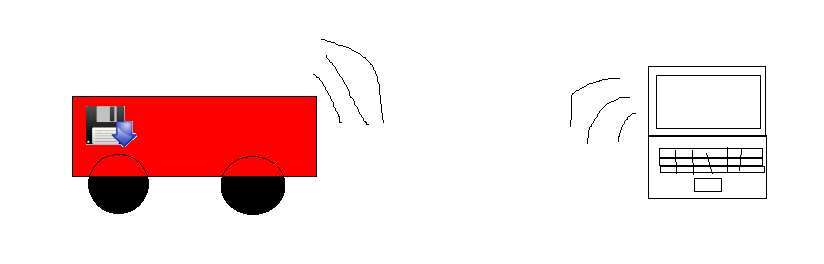
\includegraphics[width=0.6\textwidth]{graphics/go_kart_network_simple}
    \caption{SDU go-kart transferring data to a stationary computer wirelessly.}
    \label{fig:simple}
\end{figure}

While the system should be able to provide a live feed of the data being collected on the system, it should also log all data during a drive, with the possibility of transferring it later.
This will enable the user to do more advanced data analysis on the dataset than what can be achieved by monitoring the data.
In some cases, certain parameters may be irrelevant to the test being performed.
Transmitting these parameters should be avoidable by providing the possibility to start and stop data collection from specific data producers.

\begin{figure}[h]
 	\centering
    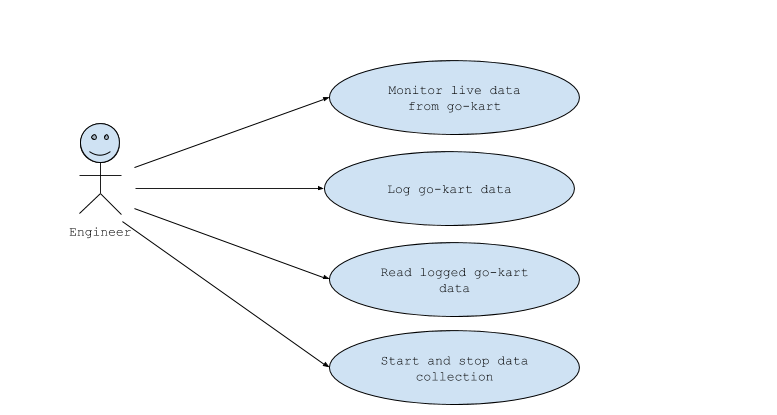
\includegraphics[width=1\textwidth]{graphics/use_cases}
    \caption{Use case diagram for the system.}
    \label{fig:usecases}
\end{figure}

As the goal of this system is to ease development on the go-kart, it should not only ease data collection, but also allow for simple addition of new sensors or other equipment.
Different projects may also have different requirements in terms of the presentation of data.
For this reason it should be possible to add a custom (G)UI of the projects design.
These requirements introduces a distinction between the actors expected to work with the system, the user and the developer.
The user will use the system to extract data from the system.
The developer will work on integrating new data producers into the system.
A use case narrative for each of the use cases is shown in appendix \ref{app:usecase}.